\documentclass{article}[twocolumn]
\usepackage[pdftex]{graphicx}
\usepackage[utf8]{inputenc}
\usepackage[brazil]{babel}
\usepackage{subfigure}
\usepackage{mathtools}
\usepackage{amsmath}
\usepackage{amssymb}
\usepackage{float}
\usepackage{tikz}

\title{Lab 3 - \textit{Sorting}}
\author{Kenji Yamane}

\begin{document}
	\maketitle
	\section{Compara\c{c}\~oes das melhores vers\~oes de cada algoritmo}
	Considerou-se para cada \textit{sorting algorithm} a seguinte vers\~ao:
	\begin{itemize}
		\item \textit{Radix Sort}: utilizou-se uma m\'ascara de 5 bits, e opera\c{c}\~oes
		\textit{bitwise} sempre que poss\'ivel.
		\item \textit{Merge Sort}: utilizou-se sua vers\~ao iterativa.
		\item \textit{Quick Sort}: utilizou-se sua vers\~ao de uma \'unica recurs\~ao, com mediana
		como piv\^o.
		\item \textit{Stl Sort}: escolhido pelo professor.
	\end{itemize}
	Com estas vers\~oes, obteve-se a figura \ref{fig:overall}.
	\begin{figure}[H]
		\centering
		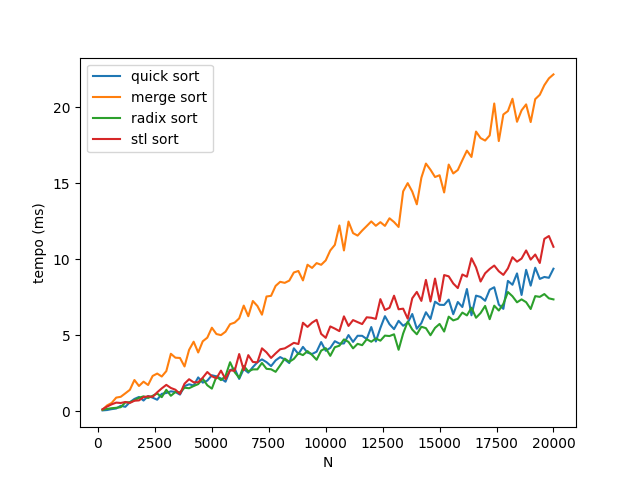
\includegraphics[width=10cm]{overall.png}
		\caption{Compara\c{c}\~ao entre as melhores vers\~oes de cada algoritmo.}
		\label{fig:overall}
	\end{figure}
	Observa-se como o \textit{radix sort} possuiu o melhor desempenho de todos, o que pode ser
	um pouco curioso dadas suas constantes grandes. Por\'em isso decorre de se ter utilizado
	uma m\'ascara bem grande. Escolheu-se sacrificar espa\c{c}o para poder ganhar no tempo,
	o cl\'assico \textit{trade-off} espa\c{c}o-tempo. A implementa\c{c}\~ao cuidadosa com somente
	operadores \textit{bit-wise} deve ter ajudado para esse resultado tamb\'em. Isso evidencia
	como o \textit{radix sort} pode ser sim o melhor algoritmo, em determinadas condi\c{c}\~oes.
	O ponto \'e que s\~ao poucas essas condi\c{c}\~oes: o algoritmo n\~ao funcionaria se tivessem
	n\'umeros negativos ou flutuantes, e teria pior desempenho se os n\'umeros fossem maiores.

	O \textit{merge sort} possuiu o pior desempenho de todos, o que \'e esperado, de acordo com
	o previsto pela teoria, sua constante multiplicativa \'e maior. Enquanto isso, o \textit{sort}
	da STL possuiu pior desempenho que o \textit{quick sort} e o \textit{radix sort}, o que pode
	ser justificado naturalmente por sua implementa\c{c}\~ao ser mais geral.

	\section{Compara\c{c}\~oes entre \textit{merge sort} recursivo e iterativo}
	Comparando-se essas duas vers\~oes do \textit{merge sort}, obt\'em-se a figura
	\ref{fig:merges}.
	\begin{figure}[H]
		\centering
		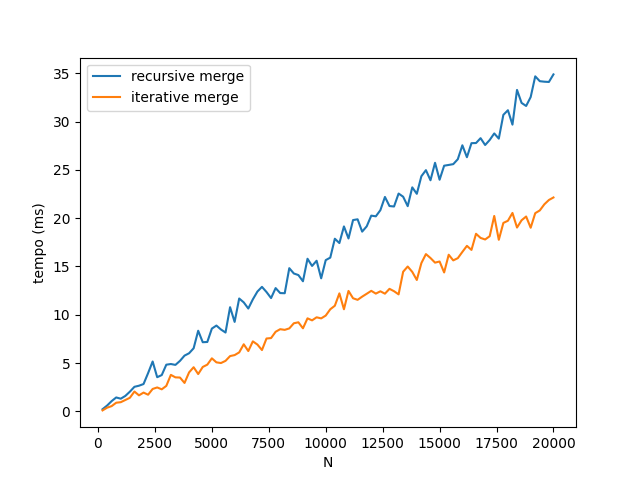
\includegraphics[width=10cm]{mergesorts.png}
		\caption{Compara\c{c}\~ao entre os \textit{merge sorts}.}
		\label{fig:merges}
	\end{figure}
	Onde se observa novamente uma acord\^ancia com a teoria. O algoritmo recursivo apresenta
	desempenho pior, o que evidencia o efeito das chamadas recursivas.

	\section{Compara\c{c}\~oes entre os \textit{quick sorts}}
	Comparou-se as seguintes vers\~oes de \textit{quick sorts}:
	\begin{itemize}
		\item \textit{Quick sort} com uma recurs\~ao e piv\^o por mediana (``o melhor'').
		\item \textit{Quick sort} com duas recurs\~oes e piv\^o por mediana.
		\item \textit{Quick sort} com duas recurs\~oes e piv\^o por ponto fixo.
	\end{itemize}
	Com estas vers\~oes, obteve-se a figura \ref{fig:quicks}.
	\begin{figure}[H]
		\centering
		\subfigure[Por tempo.]{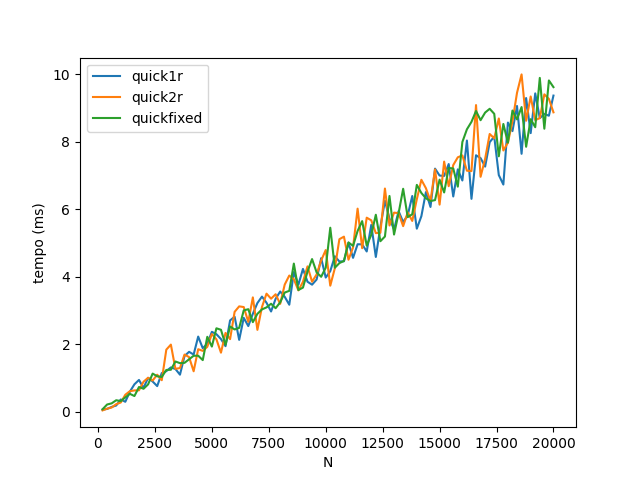
\includegraphics[width=6cm]{quicksorts_time.png}}
		\subfigure[Por chamadas.]{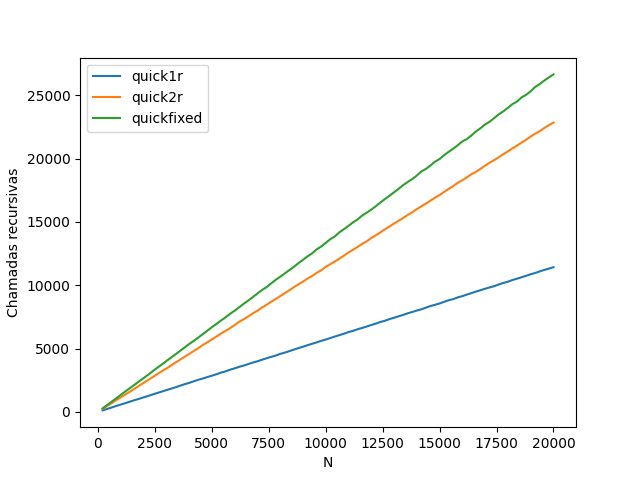
\includegraphics[width=6cm]{quicksorts_calls.png}}
		\subfigure[Por profundidade.]{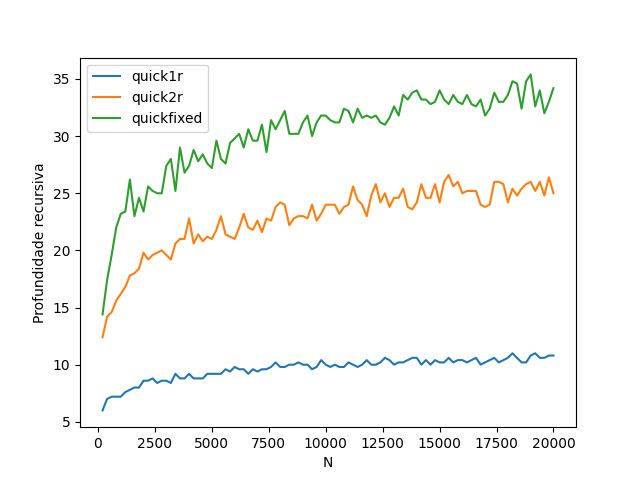
\includegraphics[width=6cm]{quicksorts_depth.png}}
		\caption{Compara\c{c}\~ao entre os \textit{quick sorts}.}
		\label{fig:quicks}
	\end{figure}
	Aqui se observa um padr\~ao que difere do previsto na teoria: claramente o melhor
	\textit{quick sort} possui bem menos recurs\~oes que o \textit{quick sort} por duas
	recurs\~oes com piv\^o por mediana, e este por sua vez possui bem menos recurs\~oes
	que o \textit{quick sort} por ponto fixo. Entretanto, isso n\~ao parece afetar o tempo
	de execu\c{c}\~ao. Recurs\~ao possui uma probabilidade mais alta de ser mais lento
	que itera\c{c}\~ao, por\'em n\~ao \'e lei. Isso n\~ao muda o fato de que as recurs\~oes
	excessivas dos algoritmos mais pobres ainda usa mais espa\c{c}o e possui mais risco
	de \textit{stack overflow}.

	\section{Compara\c{c}\~oes entre um piv\^o por mediana e um piv\^o fixo}
	Comparou-se as seguintes vers\~oes de \textit{quick sorts}:
	\begin{itemize}
		\item \textit{Quick sort} com duas recurs\~oes e piv\^o por mediana.
		\item \textit{Quick sort} com duas recurs\~oes e piv\^o por ponto fixo.
	\end{itemize}
	Os dois com vetores de \textit{input} quase ordenados, que ataca o segundo algoritmo.

	Com estas vers\~oes, obteve-se a figura \ref{fig:medianfixed}.
	\begin{figure}[H]
		\centering
		\subfigure[Por tempo.]{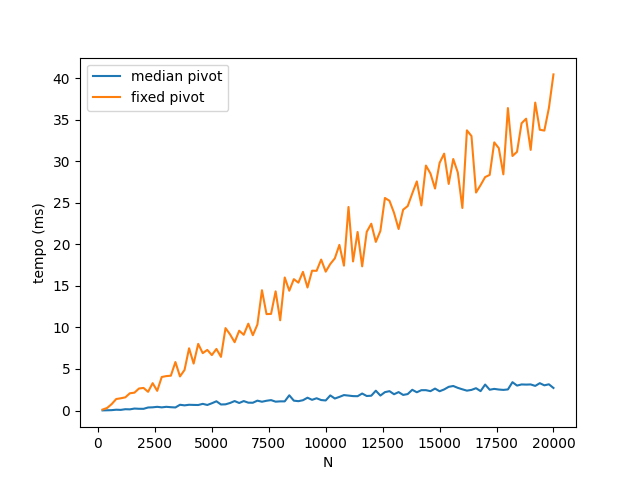
\includegraphics[width=6cm]{medianfixed_time.png}}
		\subfigure[Por chamadas.]{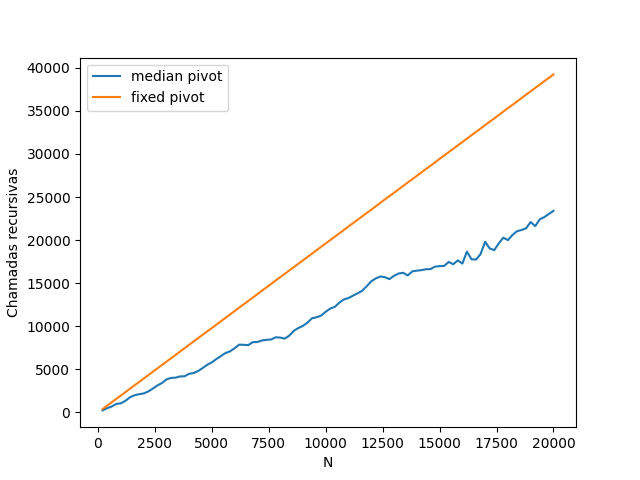
\includegraphics[width=6cm]{medianfixed_calls.png}}
		\subfigure[Por profundidade.]{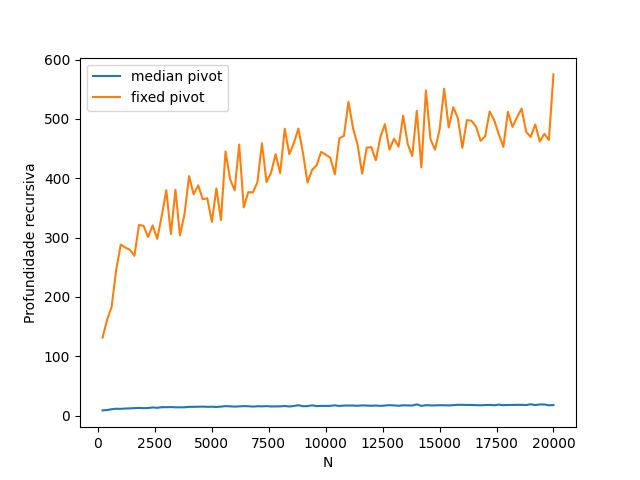
\includegraphics[width=6cm]{medianfixed_depth.png}}
		\subfigure[Profundidade por piv\^o mediano.]{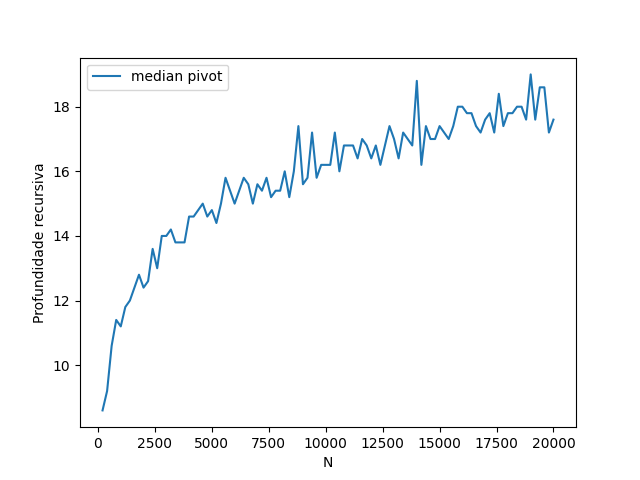
\includegraphics[width=6cm]{only_median.png}}
		\caption{Compara\c{c}\~ao entre piv\^o por mediana e o piv\^o por ponto fixo.}
		\label{fig:medianfixed}
	\end{figure}
	De fato, aqui tudo transcorre como previsto pela teoria. O piv\^o por ponto fixo \'e pobre
	em lidar com vetores quase ordenados, pois chama desnecessariamente v\'arias recurs\~oes.
	Por\'em, reitera-se como pode-se deduzir que esse pior desempenho do piv\^o por ponto fixo
	\'e por sua inefici\^encia, n\~ao por ser recursivo ao inv\'es de iterativo, dado o que
	se verificou na \'ultima se\c{c}\~ao.

	\section{Compara\c{c}\~oes entre o melhor \textit{quick sort} e o \textit{sort} do STL}
	Comparou-se o ``melhor'' \textit{quick sort} com o da STL.
	Os dois com vetores de \textit{input} quase ordenados.

	Com estas vers\~oes, obteve-se a figura \ref{fig:best}.
	\begin{figure}[H]
		\centering
		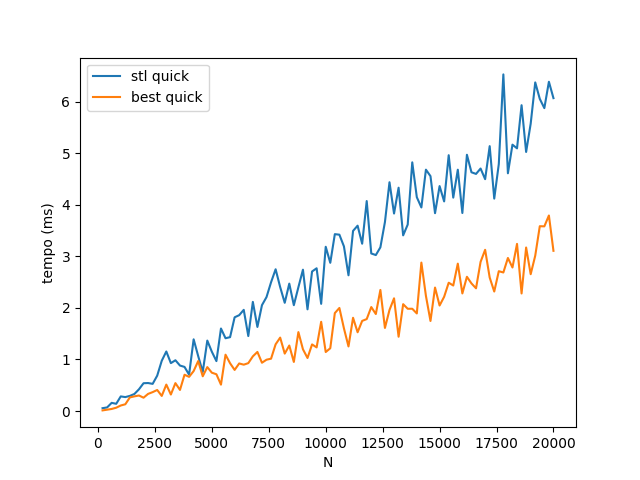
\includegraphics[width=10cm]{beststl_time.png}
		\caption{Compara\c{c}\~ao entre o ``melhor'' \textit{quick sort} e o da STL.}
		\label{fig:best}
	\end{figure}
	Novamente, como o \textit{sort} da STL \'e mais gen\'erico, ele perde para o \textit{quick
	sort} mesmo com vetores quase ordenados.
	\section{Quest\~ao opinativa}
	N\~ao \'e nada plaus\'ivel assumir que uma biblioteca como a libc escolha um algoritmo
	que fosse de complexidade quadr\'atica para os casos que essa pessoa assume. Se fosse assim,
	v\'arias comunidades estariam utilizando um algoritmo ineficiente. Ao inv\'es disso \'e
	bem mais razo\'avel assumir que eles se preocuparam em desenvolver o melhor \textit{quick
	sort} poss\'ivel que evita esses casos, como se sabe muito bem que \'e poss\'ivel. Priorizar
	uma implementa\c{c}\~ao mais f\'acil \`a otimiza\c{c}\~ao do algoritmo e efici\^encia
	num projeto como uma biblioteca a ser usada indefinidamente \'e uma atitude que somente
	um inexperiente e leigo faria.
\end{document}
